\chapter{Árboles de expansión}

\index{spanning tree}

Un \key{árbol de expansión} de un grafo consta de
todos los nodos del grafo y algunas de las
aristas del grafo de modo que haya un camino
entre dos nodos cualesquiera.
Como los árboles en general, los árboles de expansión son
conexos y acíclicos.
Normalmente hay varias formas de construir un árbol de expansión.

Por ejemplo, considera el siguiente grafo:
\begin{center}
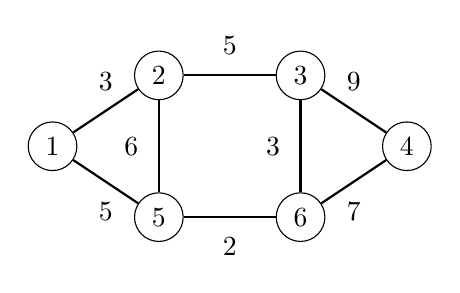
\begin{tikzpicture}[scale=0.9]
\node[draw, circle] (1) at (1.5,2) {$1$};
\node[draw, circle] (2) at (3,3) {$2$};
\node[draw, circle] (3) at (5,3) {$3$};
\node[draw, circle] (4) at (6.5,2) {$4$};
\node[draw, circle] (5) at (3,1) {$5$};
\node[draw, circle] (6) at (5,1) {$6$};
\path[draw,thick,-] (1) -- node[font=\small,label=above:3] {} (2);
\path[draw,thick,-] (2) -- node[font=\small,label=above:5] {} (3);
\path[draw,thick,-] (3) -- node[font=\small,label=above:9] {} (4);
\path[draw,thick,-] (1) -- node[font=\small,label=below:5] {} (5);
\path[draw,thick,-] (5) -- node[font=\small,label=below:2] {} (6);
\path[draw,thick,-] (6) -- node[font=\small,label=below:7] {} (4);
\path[draw,thick,-] (2) -- node[font=\small,label=left:6] {} (5);
\path[draw,thick,-] (3) -- node[font=\small,label=left:3] {} (6);
\end{tikzpicture}
\end{center}
Un árbol de expansión para el grafo es el siguiente:
\begin{center}
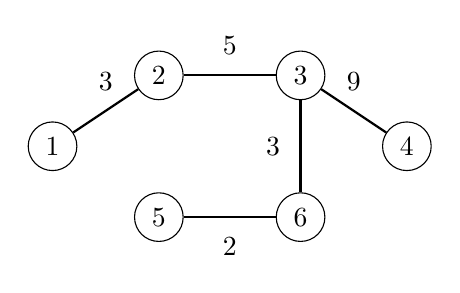
\begin{tikzpicture}[scale=0.9]
\node[draw, circle] (1) at (1.5,2) {$1$};
\node[draw, circle] (2) at (3,3) {$2$};
\node[draw, circle] (3) at (5,3) {$3$};
\node[draw, circle] (4) at (6.5,2) {$4$};
\node[draw, circle] (5) at (3,1) {$5$};
\node[draw, circle] (6) at (5,1) {$6$};
\path[draw,thick,-] (1) -- node[font=\small,label=above:3] {} (2);
\path[draw,thick,-] (2) -- node[font=\small,label=above:5] {} (3);
\path[draw,thick,-] (3) -- node[font=\small,label=above:9] {} (4);
\path[draw,thick,-] (5) -- node[font=\small,label=below:2] {} (6);
\path[draw,thick,-] (3) -- node[font=\small,label=left:3] {} (6);
\end{tikzpicture}
\end{center}

El peso de un árbol de expansión es la suma de los pesos de sus aristas.
Por ejemplo, el peso del árbol de expansión anterior es
$3+5+9+3+2=22$.

\index{minimum spanning tree}

Un \key{árbol de expansión mínima}
es un árbol de expansión cuyo peso es lo más pequeño posible.
El peso de un árbol de expansión mínima para el grafo de ejemplo
es 20, y ese árbol se puede construir de la siguiente manera:

\begin{center}
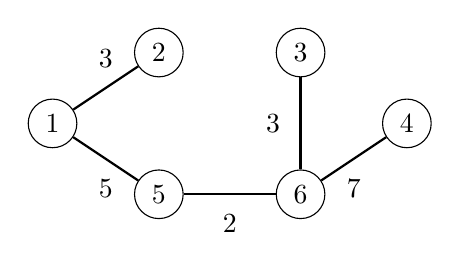
\begin{tikzpicture}[scale=0.9]
\node[draw, circle] (1) at (1.5,2) {$1$};
\node[draw, circle] (2) at (3,3) {$2$};
\node[draw, circle] (3) at (5,3) {$3$};
\node[draw, circle] (4) at (6.5,2) {$4$};
\node[draw, circle] (5) at (3,1) {$5$};
\node[draw, circle] (6) at (5,1) {$6$};

\path[draw,thick,-] (1) -- node[font=\small,label=above:3] {} (2);
\path[draw,thick,-] (1) -- node[font=\small,label=below:5] {} (5);
\path[draw,thick,-] (5) -- node[font=\small,label=below:2] {} (6);
\path[draw,thick,-] (6) -- node[font=\small,label=below:7] {} (4);
\path[draw,thick,-] (3) -- node[font=\small,label=left:3] {} (6);
\end{tikzpicture}
\end{center}

\index{maximum spanning tree}

De manera similar, un \key{árbol de expansión máxima}
es un árbol de expansión cuyo peso es lo más grande posible.
El peso de un árbol de expansión máxima para el
grafo de ejemplo es 32:

\begin{center}
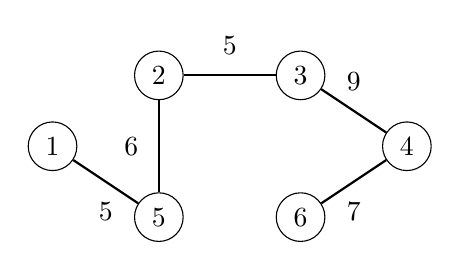
\begin{tikzpicture}[scale=0.9]
\node[draw, circle] (1) at (1.5,2) {$1$};
\node[draw, circle] (2) at (3,3) {$2$};
\node[draw, circle] (3) at (5,3) {$3$};
\node[draw, circle] (4) at (6.5,2) {$4$};
\node[draw, circle] (5) at (3,1) {$5$};
\node[draw, circle] (6) at (5,1) {$6$};
\path[draw,thick,-] (2) -- node[font=\small,label=above:5] {} (3);
\path[draw,thick,-] (3) -- node[font=\small,label=above:9] {} (4);
\path[draw,thick,-] (1) -- node[font=\small,label=below:5] {} (5);
\path[draw,thick,-] (6) -- node[font=\small,label=below:7] {} (4);
\path[draw,thick,-] (2) -- node[font=\small,label=left:6] {} (5);
\end{tikzpicture}
\end{center}

Ten en cuenta que un grafo puede tener varios
árboles de expansión mínima y máxima,
por lo que los árboles no son únicos.

Resulta que se pueden usar varios métodos voraces
para construir árboles de expansión mínima y máxima.
En este capítulo, tratamos dos algoritmos
que procesan
las aristas del grafo ordenadas por sus pesos.
Nos centramos en encontrar árboles de expansión mínima,
pero los mismos algoritmos pueden encontrar
árboles de expansión máxima procesando las aristas en orden inverso.

\section{Algoritmo de Kruskal}

\index{Kruskal's algorithm}

En el \key{algoritmo de Kruskal}\footnote{El algoritmo fue publicado en 1956
por J. B. Kruskal \cite{kru56}.}, el árbol de expansión inicial
solo contiene los nodos del grafo
y no contiene ninguna arista.
Luego, el algoritmo recorre las aristas
ordenadas por sus pesos, y siempre añade una arista
al árbol si no crea un ciclo.

El algoritmo mantiene los componentes
del árbol.
Inicialmente, cada nodo del grafo
pertenece a un componente distinto.
Siempre que se añade una arista al árbol,
se unen dos componentes.
Finalmente, todos los nodos pertenecen al mismo componente,
y se ha encontrado un árbol de expansión mínima.

\subsubsection{Ejemplo}

\begin{samepage}
Consideremos cómo el algoritmo de Kruskal procesa el
siguiente grafo:
\begin{center}
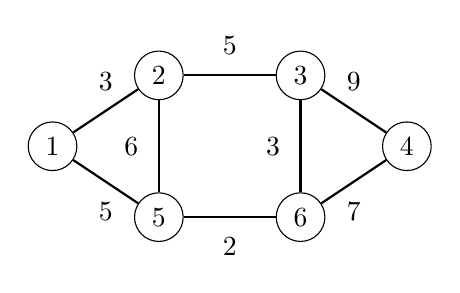
\begin{tikzpicture}[scale=0.9]
\node[draw, circle] (1) at (1.5,2) {$1$};
\node[draw, circle] (2) at (3,3) {$2$};
\node[draw, circle] (3) at (5,3) {$3$};
\node[draw, circle] (4) at (6.5,2) {$4$};
\node[draw, circle] (5) at (3,1) {$5$};
\node[draw, circle] (6) at (5,1) {$6$};
\path[draw,thick,-] (1) -- node[font=\small,label=above:3] {} (2);
\path[draw,thick,-] (2) -- node[font=\small,label=above:5] {} (3);
\path[draw,thick,-] (3) -- node[font=\small,label=above:9] {} (4);
\path[draw,thick,-] (1) -- node[font=\small,label=below:5] {} (5);
\path[draw,thick,-] (5) -- node[font=\small,label=below:2] {} (6);
\path[draw,thick,-] (6) -- node[font=\small,label=below:7] {} (4);
\path[draw,thick,-] (2) -- node[font=\small,label=left:6] {} (5);
\path[draw,thick,-] (3) -- node[font=\small,label=left:3] {} (6);
\end{tikzpicture}
\end{center}
\end{samepage}

\begin{samepage}
El primer paso del algoritmo es ordenar las
aristas en orden creciente de sus pesos.
El resultado es la siguiente lista:

\begin{tabular}{ll}
\\
arista & peso \\
\hline
5--6 & 2 \\
1--2 & 3 \\
3--6 & 3 \\
1--5 & 5 \\
2--3 & 5 \\
2--5 & 6 \\
4--6 & 7 \\
3--4 & 9 \\
\\
\end{tabular}
\end{samepage}

Después de esto, el algoritmo recorre la lista
y añade cada arista al árbol si une
dos componentes distintos.

Inicialmente, cada nodo está en su propio componente:

\begin{center}
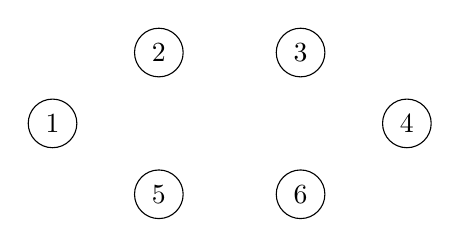
\begin{tikzpicture}[scale=0.9]
\node[draw, circle] (1) at (1.5,2) {$1$};
\node[draw, circle] (2) at (3,3) {$2$};
\node[draw, circle] (3) at (5,3) {$3$};
\node[draw, circle] (4) at (6.5,2) {$4$};
\node[draw, circle] (5) at (3,1) {$5$};
\node[draw, circle] (6) at (5,1) {$6$};
%\path[draw,thick,-] (1) -- node[font=\small,label=above:3] {} (2);
%\path[draw,thick,-] (2) -- node[font=\small,label=above:5] {} (3);
%\path[draw,thick,-] (3) -- node[font=\small,label=above:9] {} (4);
%\path[draw,thick,-] (1) -- node[font=\small,label=below:5] {} (5);
%\path[draw,thick,-] (5) -- node[font=\small,label=below:2] {} (6);
%\path[draw,thick,-] (6) -- node[font=\small,label=below:7] {} (4);
%\path[draw,thick,-] (2) -- node[font=\small,label=left:6] {} (5);
%\path[draw,thick,-] (3) -- node[font=\small,label=left:3] {} (6);
\end{tikzpicture}
\end{center}
La primera arista que se añade al árbol es
la arista 5--6 que crea un componente $\{5,6\}$
al unir los componentes $\{5\}$ y $\{6\}$:

\begin{center}
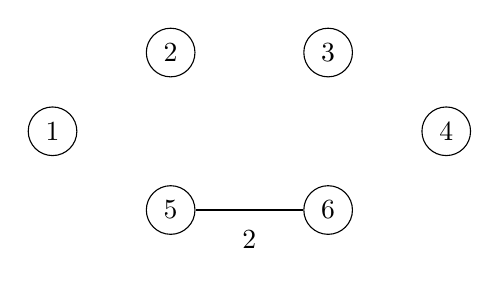
\begin{tikzpicture}
\node[draw, circle] (1) at (1.5,2) {$1$};
\node[draw, circle] (2) at (3,3) {$2$};
\node[draw, circle] (3) at (5,3) {$3$};
\node[draw, circle] (4) at (6.5,2) {$4$};
\node[draw, circle] (5) at (3,1) {$5$};
\node[draw, circle] (6) at (5,1) {$6$};

%\path[draw,thick,-] (1) -- node[font=\small,label=above:3] {} (2);
%\path[draw,thick,-] (2) -- node[font=\small,label=above:5] {} (3);
%\path[draw,thick,-] (3) -- node[font=\small,label=above:9] {} (4);
%\path[draw,thick,-] (1) -- node[font=\small,label=below:5] {} (5);
\path[draw,thick,-] (5) -- node[font=\small,label=below:2] {} (6);
%\path[draw,thick,-] (6) -- node[font=\small,label=below:7] {} (4);
%\path[draw,thick,-] (2) -- node[font=\small,label=left:6] {} (5);
%\path[draw,thick,-] (3) -- node[font=\small,label=left:3] {} (6);
\end{tikzpicture}
\end{center}
Después de esto, las aristas 1--2, 3--6 y 1--5 se añaden de manera similar:

\begin{center}
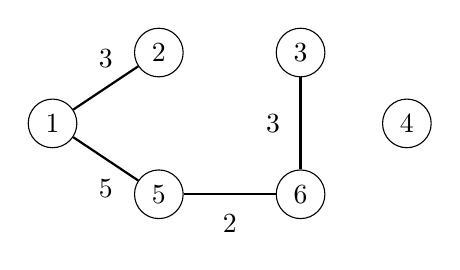
\begin{tikzpicture}[scale=0.9]
\node[draw, circle] (1) at (1.5,2) {$1$};
\node[draw, circle] (2) at (3,3) {$2$};
\node[draw, circle] (3) at (5,3) {$3$};
\node[draw, circle] (4) at (6.5,2) {$4$};
\node[draw, circle] (5) at (3,1) {$5$};
\node[draw, circle] (6) at (5,1) {$6$};

\path[draw,thick,-] (1) -- node[font=\small,label=above:3] {} (2);
%\path[draw,thick,-] (2) -- node[font=\small,label=above:5] {} (3);
%\path[draw,thick,-] (3) -- node[font=\small,label=above:9] {} (4);
\path[draw,thick,-] (1) -- node[font=\small,label=below:5] {} (5);
\path[draw,thick,-] (5) -- node[font=\small,label=below:2] {} (6);
%\path[draw,thick,-] (6) -- node[font=\small,label=below:7] {} (4);
%\path[draw,thick,-] (2) -- node[font=\small,label=left:6] {} (5);
\path[draw,thick,-] (3) -- node[font=\small,label=left:3] {} (6);
\end{tikzpicture}
\end{center}

Después de esos pasos, la mayoría de los componentes se han unido
y hay dos componentes en el árbol:
$\{1,2,3,5,6\}$ y $\{4\}$.

La siguiente arista en la lista es la arista 2--3,
pero no se incluirá en el árbol, porque
los nodos 2 y 3 ya están en el mismo componente.
Por la misma razón, la arista 2--5 no se incluirá en el árbol.

\begin{samepage}
Finalmente, la arista 4--6 se incluirá en el árbol:

\begin{center}
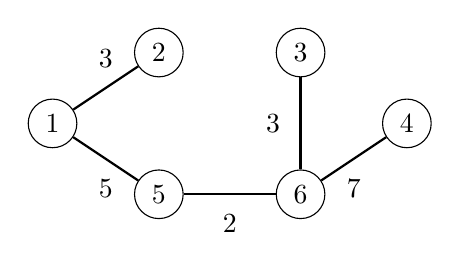
\begin{tikzpicture}[scale=0.9]
\node[draw, circle] (1) at (1.5,2) {$1$};
\node[draw, circle] (2) at (3,3) {$2$};
\node[draw, circle] (3) at (5,3) {$3$};
\node[draw, circle] (4) at (6.5,2) {$4$};
\node[draw, circle] (5) at (3,1) {$5$};
\node[draw, circle] (6) at (5,1) {$6$};

\path[draw,thick,-] (1) -- node[font=\small,label=above:3] {} (2);
%\path[draw,thick,-] (2) -- node[font=\small,label=above:5] {} (3);
%\path[draw,thick,-] (3) -- node[font=\small,label=above:9] {} (4);
\path[draw,thick,-] (1) -- node[font=\small,label=below:5] {} (5);
\path[draw,thick,-] (5) -- node[font=\small,label=below:2] {} (6);
\path[draw,thick,-] (6) -- node[font=\small,label=below:7] {} (4);
%\path[draw,thick,-] (2) -- node[font=\small,label=left:6] {} (5);
\path[draw,thick,-] (3) -- node[font=\small,label=left:3] {} (6);
\end{tikzpicture}
\end{center}
\end{samepage}

Después de esto, el algoritmo no añadirá ninguna
nueva arista, porque el grafo es conexo
y hay un camino entre dos nodos cualesquiera.
El grafo resultante es un árbol de expansión mínima
con peso $2+3+3+5+7=20$.

\subsubsection{¿Por qué funciona esto?}

Es una buena pregunta por qué funciona el algoritmo de Kruskal.
¿Por qué la estrategia voraz garantiza que
encontraremos un árbol de expansión mínima?

Veamos qué sucede si la arista de peso mínimo del
grafo \emph{no} se incluye en el árbol de expansión.
Por ejemplo, supongamos que un árbol de expansión
para el grafo anterior no contuviera la
arista de peso mínimo 5--6.
No conocemos la estructura exacta de tal árbol de expansión,
pero en cualquier caso tiene que contener algunas aristas.
Supongamos que el árbol fuera el siguiente:

\begin{center}
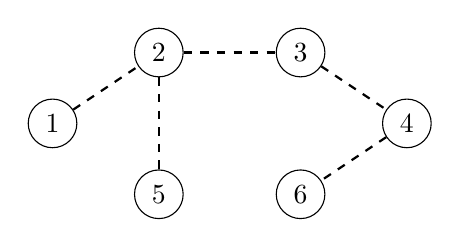
\begin{tikzpicture}[scale=0.9]
\node[draw, circle] (1) at (1.5,2) {$1$};
\node[draw, circle] (2) at (3,3) {$2$};
\node[draw, circle] (3) at (5,3) {$3$};
\node[draw, circle] (4) at (6.5,2) {$4$};
\node[draw, circle] (5) at (3,1) {$5$};
\node[draw, circle] (6) at (5,1) {$6$};

\path[draw,thick,-,dashed] (1) -- (2);
\path[draw,thick,-,dashed] (2) -- (5);
\path[draw,thick,-,dashed] (2) -- (3);
\path[draw,thick,-,dashed] (3) -- (4);
\path[draw,thick,-,dashed] (4) -- (6);
\end{tikzpicture}
\end{center}

Sin embargo, no es posible que el árbol anterior
sea un árbol de expansión mínima para el grafo.
La razón de esto es que podemos eliminar una arista
del árbol y reemplazarla con la arista de peso mínimo 5--6.
Esto produce un árbol de expansión cuyo peso es
\emph{menor}:

\begin{center}
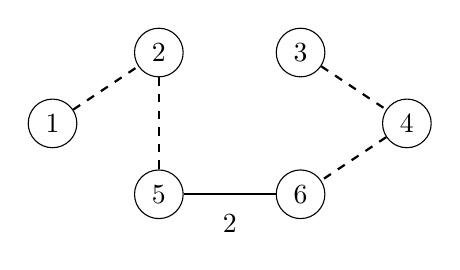
\begin{tikzpicture}[scale=0.9]
\node[draw, circle] (1) at (1.5,2) {$1$};
\node[draw, circle] (2) at (3,3) {$2$};
\node[draw, circle] (3) at (5,3) {$3$};
\node[draw, circle] (4) at (6.5,2) {$4$};
\node[draw, circle] (5) at (3,1) {$5$};
\node[draw, circle] (6) at (5,1) {$6$};

\path[draw,thick,-,dashed] (1) -- (2);
\path[draw,thick,-,dashed] (2) -- (5);
\path[draw,thick,-,dashed] (3) -- (4);
\path[draw,thick,-,dashed] (4) -- (6);
\path[draw,thick,-] (5) -- node[font=\small,label=below:2] {} (6);
\end{tikzpicture}
\end{center}

Por esta razón, siempre es óptimo
incluir la arista de peso mínimo
en el árbol para producir un árbol de expansión mínima.
Usando un argumento similar, podemos demostrar que también
es óptimo añadir al árbol la siguiente arista en orden de peso,
y así sucesivamente.
Por tanto, el algoritmo de Kruskal funciona correctamente y
siempre produce un árbol de expansión mínima.

\subsubsection{Implementación}

Al implementar el algoritmo de Kruskal,
es conveniente usar
la representación del grafo como lista de aristas.
La primera fase del algoritmo ordena las
aristas de la lista en tiempo $O(m \log m)$.
Después de esto, la segunda fase del algoritmo
construye el árbol de expansión mínima de la siguiente manera:

\begin{lstlisting}
for (...) {
  if (!same(a,b)) unite(a,b);
}
\end{lstlisting}

El bucle recorre las aristas de la lista
y siempre procesa una arista $a$--$b$
donde $a$ y $b$ son dos nodos.
Se necesitan dos funciones:
la función \texttt{same} determina
si $a$ y $b$ están en el mismo componente,
y la función \texttt{unite}
une los componentes que contienen a $a$ y $b$.

El problema es cómo implementar eficientemente
las funciones \texttt{same} y \texttt{unite}.
Una posibilidad es implementar la función
\texttt{same} como un recorrido del grafo y comprobar si
podemos llegar del nodo $a$ al nodo $b$.
Sin embargo, la complejidad temporal de tal función
sería $O(n+m)$
y el algoritmo resultante sería lento,
porque la función \texttt{same} se llamará para cada arista del grafo.

Resolveremos el problema usando una estructura union-find
que implementa ambas funciones en tiempo $O(\log n)$.
Así, la complejidad temporal del algoritmo de Kruskal
será $O(m \log n)$ después de ordenar la lista de aristas.

\section{Estructura union-find}

\index{union-find structure}

Una \key{estructura union-find} mantiene
una colección de conjuntos.
Los conjuntos son disjuntos, por lo que ningún elemento
pertenece a más de un conjunto.
Se admiten dos operaciones de tiempo $O(\log n)$:
la operación \texttt{unite} une dos conjuntos,
y la operación \texttt{find} encuentra el representante
del conjunto que contiene un elemento dado\footnote{La estructura presentada aquí
fue introducida en 1971 por J. D. Hopcroft y J. D. Ullman \cite{hop71}.
Más tarde, en 1975, R. E. Tarjan estudió una variante más sofisticada
de la estructura \cite{tar75} que se trata hoy en día en muchos
libros de texto de algoritmos.}.

\subsubsection{Estructura}

En una estructura union-find, un elemento de cada conjunto
es el representante del conjunto,
y hay una cadena desde cualquier otro elemento del
conjunto hasta el representante.
Por ejemplo, supongamos que los conjuntos son
$\{1,4,7\}$, $\{5\}$ y $\{2,3,6,8\}$:
\begin{center}
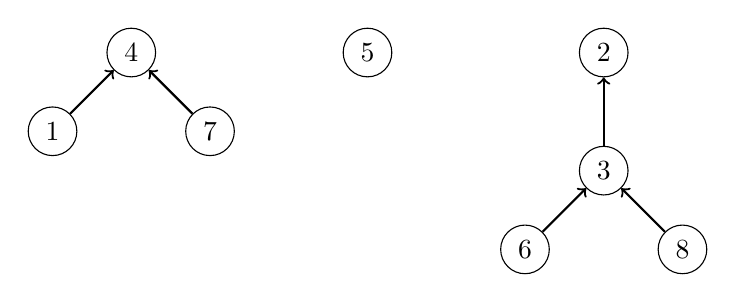
\begin{tikzpicture}
\node[draw, circle] (1) at (0,-1) {$1$};
\node[draw, circle] (2) at (7,0) {$2$};
\node[draw, circle] (3) at (7,-1.5) {$3$};
\node[draw, circle] (4) at (1,0) {$4$};
\node[draw, circle] (5) at (4,0) {$5$};
\node[draw, circle] (6) at (6,-2.5) {$6$};
\node[draw, circle] (7) at (2,-1) {$7$};
\node[draw, circle] (8) at (8,-2.5) {$8$};

\path[draw,thick,->] (1) -- (4);
\path[draw,thick,->] (7) -- (4);

\path[draw,thick,->] (3) -- (2);
\path[draw,thick,->] (6) -- (3);
\path[draw,thick,->] (8) -- (3);

\end{tikzpicture}
\end{center}
En este caso, los representantes
de los conjuntos son 4, 5 y 2.
Podemos encontrar el representante de cualquier elemento
siguiendo la cadena que comienza en el elemento.
Por ejemplo, el elemento 2 es el representante
del elemento 6, porque
seguimos la cadena $6 \rightarrow 3 \rightarrow 2$.
Dos elementos pertenecen al mismo conjunto exactamente cuando
sus representantes son iguales.

Dos conjuntos se pueden unir conectando el
representante de un conjunto al
representante del otro conjunto.
Por ejemplo, los conjuntos
$\{1,4,7\}$ y $\{2,3,6,8\}$
se pueden unir de la siguiente manera:
\begin{center}
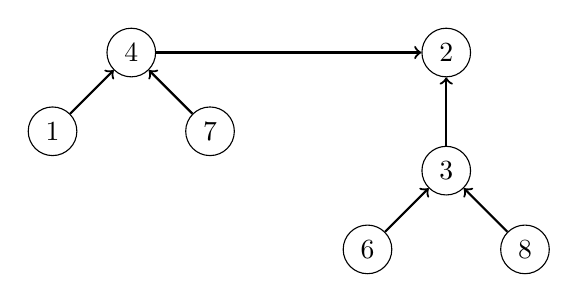
\begin{tikzpicture}
\node[draw, circle] (1) at (2,-1) {$1$};
\node[draw, circle] (2) at (7,0) {$2$};
\node[draw, circle] (3) at (7,-1.5) {$3$};
\node[draw, circle] (4) at (3,0) {$4$};
\node[draw, circle] (6) at (6,-2.5) {$6$};
\node[draw, circle] (7) at (4,-1) {$7$};
\node[draw, circle] (8) at (8,-2.5) {$8$};

\path[draw,thick,->] (1) -- (4);
\path[draw,thick,->] (7) -- (4);

\path[draw,thick,->] (3) -- (2);
\path[draw,thick,->] (6) -- (3);
\path[draw,thick,->] (8) -- (3);

\path[draw,thick,->] (4) -- (2);
\end{tikzpicture}
\end{center}

El conjunto resultante contiene los elementos
$\{1,2,3,4,6,7,8\}$.
A partir de ahora, el elemento 2 es el representante
de todo el conjunto y el antiguo representante 4
apunta al elemento 2.

La eficiencia de la estructura union-find depende de
cómo se unan los conjuntos.
Resulta que podemos seguir una estrategia sencilla:
conectar siempre el representante del
conjunto \emph{menor} al representante del conjunto \emph{mayor}
(o si los conjuntos son de igual tamaño,
podemos hacer una elección arbitraria).
Usando esta estrategia, la longitud de cualquier cadena
será $O(\log n)$, por lo que podemos
encontrar el representante de cualquier elemento
eficientemente siguiendo la cadena correspondiente.

\subsubsection{Implementación}

La estructura union-find se puede implementar
usando arreglos.
En la siguiente implementación,
el arreglo \texttt{link} contiene para cada elemento
el siguiente elemento
de la cadena o el elemento mismo si es
un representante,
y el arreglo \texttt{size} indica para cada representante
el tamaño del conjunto correspondiente.

Inicialmente, cada elemento pertenece a un conjunto distinto:
\begin{lstlisting}
for (int i = 1; i <= n; i++) link[i] = i;
for (int i = 1; i <= n; i++) size[i] = 1;
\end{lstlisting}

La función \texttt{find} devuelve
el representante de un elemento $x$.
El representante se puede encontrar siguiendo
la cadena que comienza en $x$.

\begin{lstlisting}
int find(int x) {
    while (x != link[x]) x = link[x];
    return x;
}
\end{lstlisting}

La función \texttt{same} comprueba
si los elementos $a$ y $b$ pertenecen al mismo conjunto.
Esto se puede hacer fácilmente usando la
función \texttt{find}:

\begin{lstlisting}
bool same(int a, int b) {
    return find(a) == find(b);
}
\end{lstlisting}

\begin{samepage}
La función \texttt{unite} une los conjuntos
que contienen los elementos $a$ y $b$
(los elementos tienen que estar en conjuntos diferentes).
La función primero encuentra los representantes
de los conjuntos y luego conecta el conjunto
menor al conjunto mayor.

\begin{lstlisting}
void unite(int a, int b) {
    a = find(a);
    b = find(b);
    if (size[a] < size[b]) swap(a,b);
    size[a] += size[b];
    link[b] = a;
}
\end{lstlisting}
\end{samepage}

La complejidad temporal de la función \texttt{find}
es $O(\log n)$ suponiendo que la longitud de cada
cadena es $O(\log n)$.
En este caso, las funciones \texttt{same} y \texttt{unite}
también funcionan en tiempo $O(\log n)$.
La función \texttt{unite} se asegura de que la
longitud de cada cadena sea $O(\log n)$ conectando
el conjunto menor al conjunto mayor.

\section{Algoritmo de Prim}

\index{Prim's algorithm}

El \key{algoritmo de Prim}\footnote{El algoritmo lleva
el nombre de R. C. Prim, quien lo publicó en 1957 \cite{pri57}.
Sin embargo, el mismo algoritmo ya había sido descubierto en 1930
por V. Jarník.} es un método alternativo
para encontrar un árbol de expansión mínima.
El algoritmo primero añade un nodo arbitrario
al árbol.
Después de esto, el algoritmo siempre elige
una arista de peso mínimo que
añade un nuevo nodo al árbol.
Finalmente, todos los nodos se han añadido al árbol
y se ha encontrado un árbol de expansión mínima.

El algoritmo de Prim se parece al algoritmo de Dijkstra.
La diferencia es que el algoritmo de Dijkstra siempre
selecciona una arista cuya distancia desde el nodo
inicial es mínima, pero el algoritmo de Prim simplemente selecciona
la arista de peso mínimo que añade un nuevo nodo al árbol.

\subsubsection{Ejemplo}

Consideremos cómo funciona el algoritmo de Prim
en el siguiente grafo:

\begin{center}
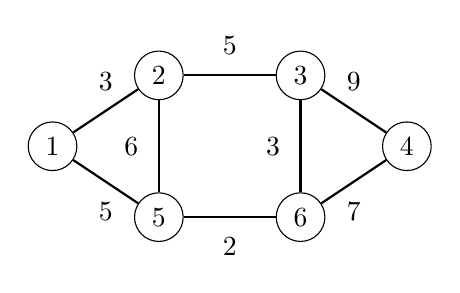
\begin{tikzpicture}[scale=0.9]
\node[draw, circle] (1) at (1.5,2) {$1$};
\node[draw, circle] (2) at (3,3) {$2$};
\node[draw, circle] (3) at (5,3) {$3$};
\node[draw, circle] (4) at (6.5,2) {$4$};
\node[draw, circle] (5) at (3,1) {$5$};
\node[draw, circle] (6) at (5,1) {$6$};
\path[draw,thick,-] (1) -- node[font=\small,label=above:3] {} (2);
\path[draw,thick,-] (2) -- node[font=\small,label=above:5] {} (3);
\path[draw,thick,-] (3) -- node[font=\small,label=above:9] {} (4);
\path[draw,thick,-] (1) -- node[font=\small,label=below:5] {} (5);
\path[draw,thick,-] (5) -- node[font=\small,label=below:2] {} (6);
\path[draw,thick,-] (6) -- node[font=\small,label=below:7] {} (4);
\path[draw,thick,-] (2) -- node[font=\small,label=left:6] {} (5);
\path[draw,thick,-] (3) -- node[font=\small,label=left:3] {} (6);

%\path[draw=red,thick,-,line width=2pt] (5) -- (6);
\end{tikzpicture}
\end{center}
Inicialmente, no hay aristas entre los nodos:
\begin{center}
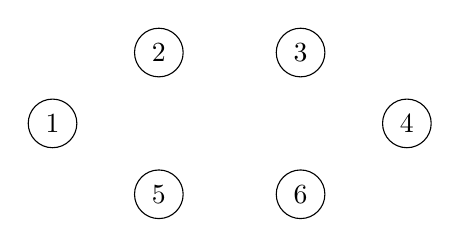
\begin{tikzpicture}[scale=0.9]
\node[draw, circle] (1) at (1.5,2) {$1$};
\node[draw, circle] (2) at (3,3) {$2$};
\node[draw, circle] (3) at (5,3) {$3$};
\node[draw, circle] (4) at (6.5,2) {$4$};
\node[draw, circle] (5) at (3,1) {$5$};
\node[draw, circle] (6) at (5,1) {$6$};
%\path[draw,thick,-] (1) -- node[font=\small,label=above:3] {} (2);
%\path[draw,thick,-] (2) -- node[font=\small,label=above:5] {} (3);
%\path[draw,thick,-] (3) -- node[font=\small,label=above:9] {} (4);
%\path[draw,thick,-] (1) -- node[font=\small,label=below:5] {} (5);
%\path[draw,thick,-] (5) -- node[font=\small,label=below:2] {} (6);
%\path[draw,thick,-] (6) -- node[font=\small,label=below:7] {} (4);
%\path[draw,thick,-] (2) -- node[font=\small,label=left:6] {} (5);
%\path[draw,thick,-] (3) -- node[font=\small,label=left:3] {} (6);
\end{tikzpicture}
\end{center}
Cualquier nodo puede ser el nodo inicial,
así que elijamos el nodo 1.
Primero, añadimos el nodo 2 que está conectado por
una arista de peso 3:
\begin{center}
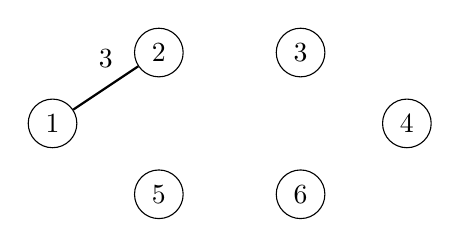
\begin{tikzpicture}[scale=0.9]
\node[draw, circle] (1) at (1.5,2) {$1$};
\node[draw, circle] (2) at (3,3) {$2$};
\node[draw, circle] (3) at (5,3) {$3$};
\node[draw, circle] (4) at (6.5,2) {$4$};
\node[draw, circle] (5) at (3,1) {$5$};
\node[draw, circle] (6) at (5,1) {$6$};
\path[draw,thick,-] (1) -- node[font=\small,label=above:3] {} (2);
%\path[draw,thick,-] (2) -- node[font=\small,label=above:5] {} (3);
%\path[draw,thick,-] (3) -- node[font=\small,label=above:9] {} (4);
%\path[draw,thick,-] (1) -- node[font=\small,label=below:5] {} (5);
%\path[draw,thick,-] (5) -- node[font=\small,label=below:2] {} (6);
%\path[draw,thick,-] (6) -- node[font=\small,label=below:7] {} (4);
%\path[draw,thick,-] (2) -- node[font=\small,label=left:6] {} (5);
%\path[draw,thick,-] (3) -- node[font=\small,label=left:3] {} (6);
\end{tikzpicture}
\end{center}

Después de esto, hay dos aristas de peso 5,
por lo que podemos añadir el nodo 3 o el nodo 5 al árbol.
Añadamos primero el nodo 3:
\begin{center}
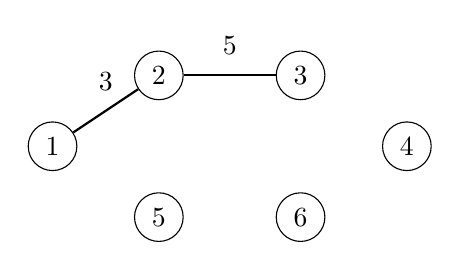
\begin{tikzpicture}[scale=0.9]
\node[draw, circle] (1) at (1.5,2) {$1$};
\node[draw, circle] (2) at (3,3) {$2$};
\node[draw, circle] (3) at (5,3) {$3$};
\node[draw, circle] (4) at (6.5,2) {$4$};
\node[draw, circle] (5) at (3,1) {$5$};
\node[draw, circle] (6) at (5,1) {$6$};
\path[draw,thick,-] (1) -- node[font=\small,label=above:3] {} (2);
\path[draw,thick,-] (2) -- node[font=\small,label=above:5] {} (3);
%\path[draw,thick,-] (3) -- node[font=\small,label=above:9] {} (4);
%\path[draw,thick,-] (1) -- node[font=\small,label=below:5] {} (5);
%\path[draw,thick,-] (5) -- node[font=\small,label=below:2] {} (6);
%\path[draw,thick,-] (6) -- node[font=\small,label=below:7] {} (4);
%\path[draw,thick,-] (2) -- node[font=\small,label=left:6] {} (5);
%\path[draw,thick,-] (3) -- node[font=\small,label=left:3] {} (6);
\end{tikzpicture}
\end{center}

\begin{samepage}
El proceso continúa hasta que todos los nodos se han incluido en el árbol:
\begin{center}
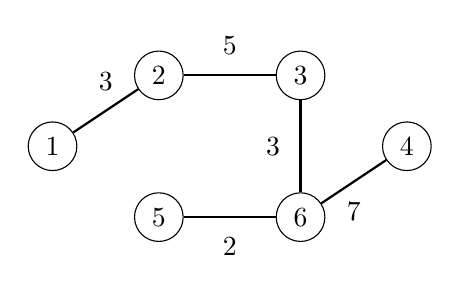
\begin{tikzpicture}[scale=0.9]
\node[draw, circle] (1) at (1.5,2) {$1$};
\node[draw, circle] (2) at (3,3) {$2$};
\node[draw, circle] (3) at (5,3) {$3$};
\node[draw, circle] (4) at (6.5,2) {$4$};
\node[draw, circle] (5) at (3,1) {$5$};
\node[draw, circle] (6) at (5,1) {$6$};
\path[draw,thick,-] (1) -- node[font=\small,label=above:3] {} (2);
\path[draw,thick,-] (2) -- node[font=\small,label=above:5] {} (3);
%\path[draw,thick,-] (3) -- node[font=\small,label=above:9] {} (4);
%\path[draw,thick,-] (1) -- node[font=\small,label=below:5] {} (5);
\path[draw,thick,-] (5) -- node[font=\small,label=below:2] {} (6);
\path[draw,thick,-] (6) -- node[font=\small,label=below:7] {} (4);
%\path[draw,thick,-] (2) -- node[font=\small,label=left:6] {} (5);
\path[draw,thick,-] (3) -- node[font=\small,label=left:3] {} (6);
\end{tikzpicture}
\end{center}
\end{samepage}

\subsubsection{Implementación}

Como el algoritmo de Dijkstra, el algoritmo de Prim se puede
implementar eficientemente usando una cola de prioridad.
La cola de prioridad debe contener todos los nodos
que se pueden conectar al componente actual usando
una sola arista, en orden creciente de los pesos
de las aristas correspondientes.

La complejidad temporal del algoritmo de Prim es
$O(n + m \log m)$ que es igual a la complejidad temporal
del algoritmo de Dijkstra.
En la práctica, los algoritmos de Prim y Kruskal
son ambos eficientes, y la elección del algoritmo
es cuestión de gustos.
Aun así, la mayoría de los programadores competitivos usan el algoritmo de Kruskal.
